Assumptions:
\begin{itemize}
    \item $g = \SI{10}{ms^{-2}}$
    \item speed limit = \SI{14}{ms^{-1}} ($\approx$ \SI{50}{km\per h})
    \item Motorcycle mass, $m_m= \SI{300}{kg}$
    \item Tree trunk mass, $m_t = \SI{100}{kg}$
\end{itemize}
\subsection*{i}

    \begin{figure}[h!]
        \centering
        \captionsetup[subfigure]{font=footnotesize}
        \subcaptionbox{Accelerating}[.48\textwidth]{
            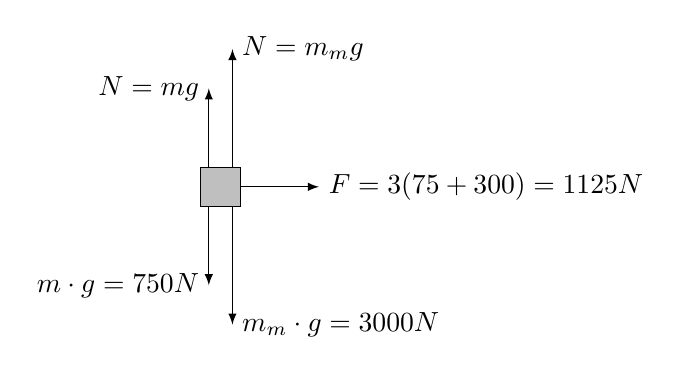
\begin{tikzpicture}
                \draw[fill=gray!50] coordinate (L) rectangle ++(0.5,-0.5)coordinate(Q);
                \draw[-latex] (L)++(0.4,-0.5) -- ++(0,-1.5)node[right]{$ m_m\cdot g = \SI{3000}{N}$};
                \draw[-latex] (L)++(0.1,-0.5) -- ++(0,-1.0)node[left]{$ m\cdot g = \SI{750}{N}$};
                \draw[-latex] (L)++(0.4,0) -- ++(0,1.5)node[right]{$N=m_m g$};
                \draw[-latex] (L)++(0.1,0) -- ++(0,1.0)node[left]{$N=m g$};
                \draw[-latex] (L)++(0.5,-0.25) -- ++(1.0,0)node[right]{$F=3(75+300) = \SI{1125}{N}$};
            \end{tikzpicture}
        }
        \subcaptionbox{Constant speed}[.48\textwidth]{
            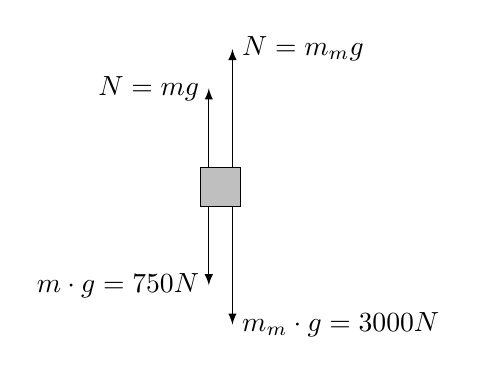
\begin{tikzpicture}
                \draw[fill=gray!50]  coordinate (L) rectangle ++(0.5,-0.5)coordinate(Q);
                \draw[-latex] (L)++(0.4,-0.5) -- ++(0,-1.5)node[right]{$ m_m\cdot g = \SI{3000}{N}$};
                \draw[-latex] (L)++(0.1,-0.5) -- ++(0,-1.0)node[left]{$ m\cdot g = \SI{750}{N}$};
                \draw[-latex] (L)++(0.4,0) -- ++(0,1.5)node[right]{$N=m_m g$};
                \draw[-latex] (L)++(0.1,0) -- ++(0,1.0)node[left]{$N=m g$};
            \end{tikzpicture}
        }
    \end{figure}

\subsection*{ii}
    \begin{equation}
        \begin{split}
            V = V_0 + at = \SI{14}{ms^{-1}} + \SI{3}{ms^{-2}} \cdot \SI{4.5}{s} \\
            V = \SI{27.5}{m\per s}
        \end{split}
    \end{equation}

\subsection*{iii}

    \subsubsection*{a)}
        \begin{equation}
            \begin{split}
                d &= \frac{V^2 - {V_0}^2}{2a} = \frac{27.5^2 - 14^2}{2\cdot 3} = \SI{93.375}{m}\\
                W &= (m+m_m) \cdot a \cdot d = \SI{375}{kg} \cdot \SI{3}{ms^{-2}} \cdot \SI{93.375}{m} \\
                W &= \SI{105046.9}{J}
            \end{split}
        \end{equation}
        
    \subsubsection*{b)}
        There are no unbalanced forces in the direction of the motion, therefore $ W = 0$.

\subsection*{iv}
    Given that it is an inelastic collision, both John and the tree trunk will have the same speed $V_f$ after collision:  
    \begin{equation}
        \begin{split}
            (m+m_m) V &= (m+ m_m + m_t) V_f \implies V_f = \frac{(m+m_m) V}{(m+ m_m + m_t)}\\
            V_f &= \frac{375 \cdot 27.5}{475} = \SI{21.7}{ms^{-1}}
        \end{split}
    \end{equation}
    Given an impulse J,
    \begin{equation}
        \begin{split}
            J = Ft = \Delta p \implies F = \frac{\Delta p}{t} \\
            F = \frac{375 \cdot (27.5 - 21.7)}{0.1} = \SI{21750}{N}
        \end{split}
    \end{equation}